\documentclass[tikz]{standalone}

\usepackage{tikz}
\usetikzlibrary{trees}
\usetikzlibrary{shapes}
\usetikzlibrary{positioning}
\usetikzlibrary{arrows.meta}

\tikzset{
    pointer/.style = {thick,draw=black,triangle 45-*,shorten >=-3pt},
    cell/.style = {rectangle, thick, draw=black,minimum width = 1cm, minimum height =1.0cm,fill=yellow!20},
    mynode/.style = {circle, thick, draw=black, align=center,fill=yellow!40,font=\ttfamily\bfseries\Large},
    mynoder/.style = {circle, thick, draw=black, align=center,fill=red!30,font=\ttfamily\bfseries\Large},
    mynodeb/.style = {circle, thick, draw=black, align=center,fill=blue!30,font=\ttfamily\bfseries\Large},
    edgen/.style = {-latex,ultra thick},
    edger/.style = {-latex,ultra thick,red},
    edgeb/.style = {-latex,ultra thick,blue},
    edgeg/.style = {-latex,ultra thick,gray},
    edgegd/.style = {-latex,ultra thick,brown,dashed}, % back
    edgevd/.style = {-latex,ultra thick,violet,dotted}, % forward
    edgexd/.style = {-latex,ultra thick,blue,densely dotted}, % traversal
    every picture/.style={/utils/exec={\ttfamily\bfseries}},
    every picture/.style={font issue=\ttfamily\bfseries},
    font issue/.style={execute at begin picture={#1\selectfont}
  }
}

\begin{document}

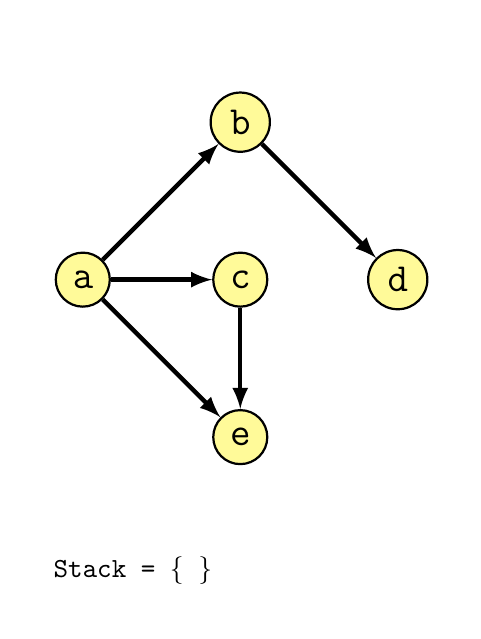
\begin{tikzpicture}[scale=1.00,transform shape]
%
\node[mynode] at (0,2) (a) {a};
\node[mynode] at (2,4) (b) {b};
\node[mynode] at (2,2) (c) {c};
\node[mynode] at (4,2) (d) {d};
\node[mynode] at (2,0) (e) {e};
%
\draw[edgen] (a) edge node {} (b);
\draw[edgen] (a) edge node {} (c);
\draw[edgen] (a) edge node {} (e);
\draw[edgen] (c) edge node {} (e);
\draw[edgen] (b) edge node {} (d);

\path[use as bounding box] (-0.7,-2.2) rectangle (4.7, 5.2);
\node[align=left,above right,draw=none] at (-0.5,-2.0) {Stack = \{  \}};

\end{tikzpicture}

\newpage
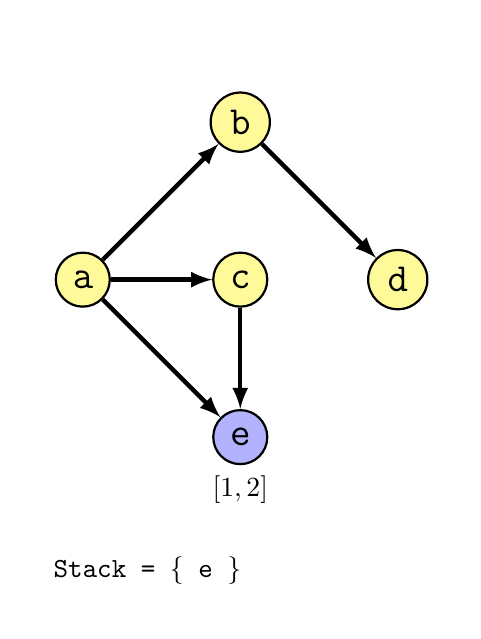
\begin{tikzpicture}[scale=1.00,transform shape]
%
\node[mynode] at (0,2) (a) {a};
\node[mynode] at (2,4) (b) {b};
\node[mynode] at (2,2) (c) {c};
\node[mynode] at (4,2) (d) {d};
\node[mynodeb,label={below:$[1, 2]$}] at (2,0) (e) {e};
%
\draw[edgen] (a) edge node {} (b);
\draw[edgen] (a) edge node {} (c);
\draw[edgen] (a) edge node {} (e);
\draw[edgen] (c) edge node {} (e);
\draw[edgen] (b) edge node {} (d);

\path[use as bounding box] (-0.7,-2.2) rectangle (4.7, 5.2);
\node[align=left,above right,draw=none] at (-0.5,-2.0) {Stack = \{ e \}};

\end{tikzpicture}

\newpage
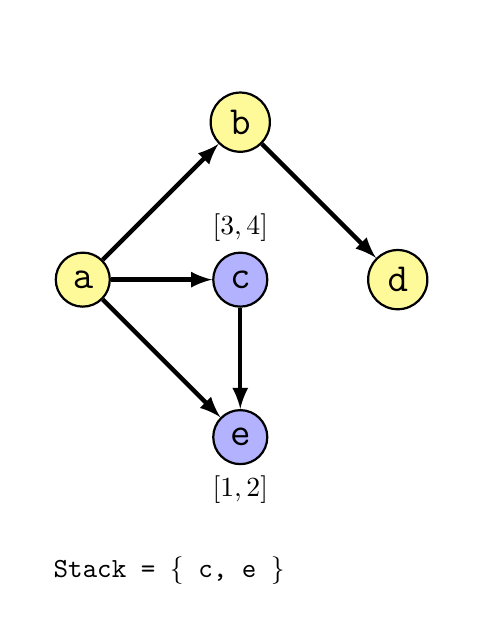
\begin{tikzpicture}[scale=1.00,transform shape]
%
\node[mynode] at (0,2) (a) {a};
\node[mynode] at (2,4) (b) {b};
\node[mynodeb,label={above:$[3, 4]$}] at (2,2) (c) {c};
\node[mynode] at (4,2) (d) {d};
\node[mynodeb,label={below:$[1, 2]$}] at (2,0) (e) {e};
%
\draw[edgen] (a) edge node {} (b);
\draw[edgen] (a) edge node {} (c);
\draw[edgen] (a) edge node {} (e);
\draw[edgen] (c) edge node {} (e);
\draw[edgen] (b) edge node {} (d);

\path[use as bounding box] (-0.7,-2.2) rectangle (4.7, 5.2);
\node[align=left,above right,draw=none] at (-0.5,-2.0) {Stack = \{ c, e \}};

\end{tikzpicture}

\newpage
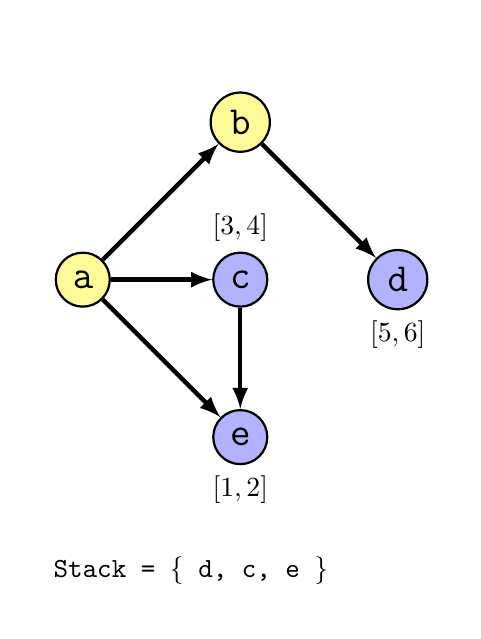
\begin{tikzpicture}[scale=1.00,transform shape]
%
\node[mynode] at (0,2) (a) {a};
\node[mynode] at (2,4) (b) {b};
\node[mynodeb,label={above:$[3, 4]$}] at (2,2) (c) {c};
\node[mynodeb,label={below:$[5, 6]$}] at (4,2) (d) {d};
\node[mynodeb,label={below:$[1, 2]$}] at (2,0) (e) {e};
%
\draw[edgen] (a) edge node {} (b);
\draw[edgen] (a) edge node {} (c);
\draw[edgen] (a) edge node {} (e);
\draw[edgen] (c) edge node {} (e);
\draw[edgen] (b) edge node {} (d);

\path[use as bounding box] (-0.7,-2.2) rectangle (4.7, 5.2);
\node[align=left,above right,draw=none] at (-0.5,-2.0) {Stack = \{ d, c, e \}};

\end{tikzpicture}

\newpage
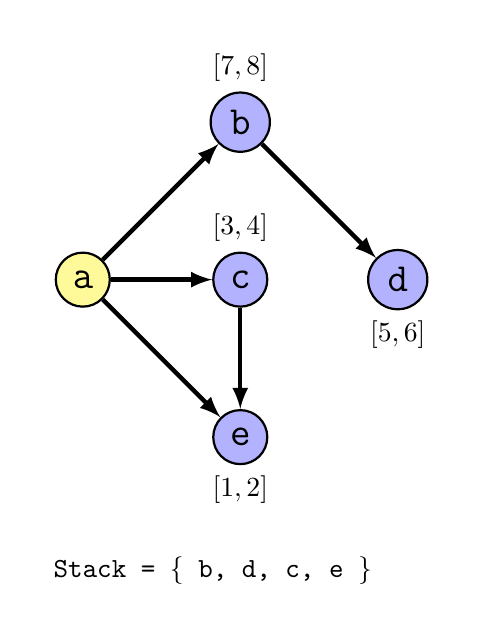
\begin{tikzpicture}[scale=1.00,transform shape]
%
\node[mynode] at (0,2) (a) {a};
\node[mynodeb,label={above:$[7, 8]$}] at (2,4) (b) {b};
\node[mynodeb,label={above:$[3, 4]$}] at (2,2) (c) {c};
\node[mynodeb,label={below:$[5, 6]$}] at (4,2) (d) {d};
\node[mynodeb,label={below:$[1, 2]$}] at (2,0) (e) {e};
%
\draw[edgen] (a) edge node {} (b);
\draw[edgen] (a) edge node {} (c);
\draw[edgen] (a) edge node {} (e);
\draw[edgen] (c) edge node {} (e);
\draw[edgen] (b) edge node {} (d);

\path[use as bounding box] (-0.7,-2.2) rectangle (4.7, 5.2);
\node[align=left,above right,draw=none] at (-0.5,-2.0) {Stack = \{ b, d, c, e \}};

\end{tikzpicture}

\newpage
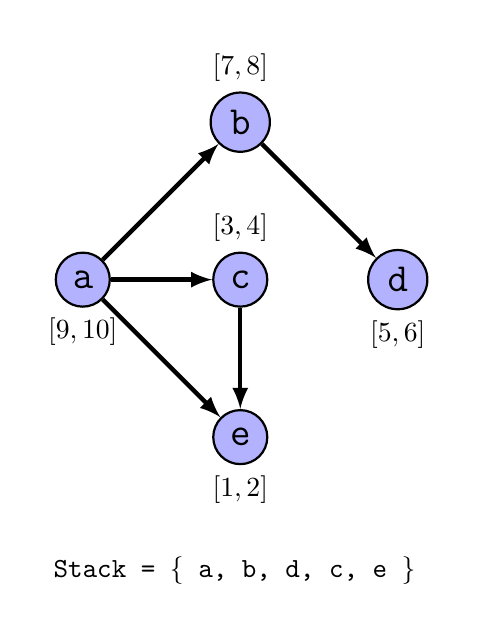
\begin{tikzpicture}[scale=1.00,transform shape]
%
\node[mynodeb,label={below:$[9, 10]$}] at (0,2) (a) {a};
\node[mynodeb,label={above:$[7, 8]$}] at (2,4) (b) {b};
\node[mynodeb,label={above:$[3, 4]$}] at (2,2) (c) {c};
\node[mynodeb,label={below:$[5, 6]$}] at (4,2) (d) {d};
\node[mynodeb,label={below:$[1, 2]$}] at (2,0) (e) {e};
%
\draw[edgen] (a) edge node {} (b);
\draw[edgen] (a) edge node {} (c);
\draw[edgen] (a) edge node {} (e);
\draw[edgen] (c) edge node {} (e);
\draw[edgen] (b) edge node {} (d);

\path[use as bounding box] (-0.7,-2.2) rectangle (4.7, 5.2);
\node[align=left,above right,draw=none] at (-0.5,-2.0) {Stack = \{ a, b, d, c, e \}};

\end{tikzpicture}




\end{document}